\section{Geometria Trifocal}

\subsection{O Problema}

\subsection{Abordagem por Tensor Trifocal}

\subsection{Pesquisas Anteriores para Determinação de Câmera usando três Imagens}

\subsubsection{Abordagem do Nistér}

Para abordar um problema trifocal, primeiro \cite{2503343} desenvolvem uma abordagem num sistemna bifocal para determinação da rotação e da translação (supondo qua a calibração já seja conhecida) da segunda câmera em relação à primeira, considerando duas imagens de quatro pontos em 3D. Eles demonstram que os epipolos de cada imagem estão restritos a se alojarem numa curva de grau 10, a chamada curva décica, bem como desenvolvem um método para a obtenção dessa curva. Em seguida, utilizam essa teoria para desenvolver o que chamaram de solução mais eficiente para época (2006), o notório desafio de estabelecer as poses das câmeras num sistema com três imagens. Vamos reproduzir os detalhes mais importantes. 

\begin{figure}[!htb]
\centering
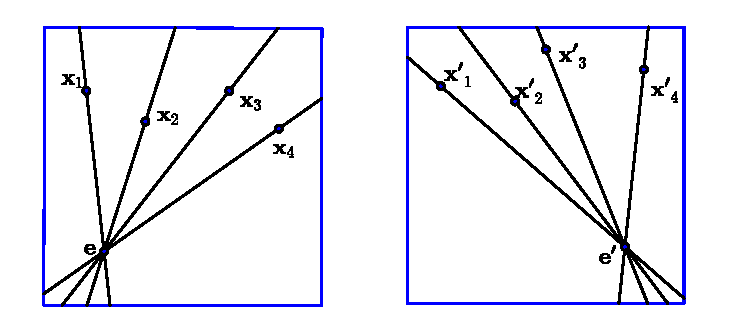
\includegraphics[scale=.85]{retas-epipolares}
\caption{\textit{Feixe de retas passando pelo epipolo em cada imagem, relacionadas duas a duas por uma homografia.}}
\label{retas-epipolares}
\end{figure}

{\bf A homografia da reta epipolar.} Dados $n$ correspondências de pontos em duas imagens, a \textit{restrição epipolar} \citep{faugeras93three} pode ser expressa como: os parâmetros projetivos das $n$ retas ligando o epipolo ${\bf e}$ aos pontos ${\bf x}_i$ na primeira imagem, estão homograficamente relacionados com os parâmetros projetivos das $n$ retas ligando o epipolo ${\bf e'}$ aos pontos ${\bf x'}_i$ na segunda imagem. Ou seja, temos uma homografia 1D que relaciona o feixe de retas através ${\bf e}$ com o feixe de retas através ${\bf e'}$ chamada \textit{homografia da reta epipolar}. Podemos visualizar essa situação na figura \ref{retas-epipolares}.


Supondo os epipolos na origem do plano de cada imagem, com as retas epipolares passando pelo epipolo, cada reta pode ser parametrizada através do ângulo que ela forma com o eixo das abscissas, denominados $\alpha_1$ e $\alpha_2$ na primeira e segunda imagens respectivamente.
A homografia da reta epipolar pode ser representada pela equação de uma hipérbole alinhada aos eixos perpendiculares, conforme descrito em \cite{Fabbri:Kimia:IJCV2015}.

\begin{equation}\label{eq.hiperbole}
a\,x\,y+b\,x+c\,y+d=0 \qquad \text{ou} \qquad y=\frac{-b\,x-d}{a\,x+c},
\end{equation} 
onde $x=tan\,\alpha_1$ e $y=tan\,\alpha_2$. 

Vemos na figura \ref{fig.reta-epipolar} que cada reta epipolar fica definida por um ponto no eixo da tangente, $(1,tan\,\alpha_1)$ na primeira imagem e $(1,tan\,\alpha_2)$ na segunda, onde consideramos o círculo trigonométrico de raio $1$. Usando esses pontos, a equação da hipérbole pode ser escrita na forma

\begin{equation}\label{eq.homo-reta-epi}
(1\,,\,tan\,\alpha_1)
\overbrace{
\begin{bmatrix}
d&c\\
b&a
\end{bmatrix}
}^{H}
\begin{pmatrix}
1\\
tan\,\alpha_2
\end{pmatrix}
=0,
\end{equation}
sendo 
$\begin{bmatrix}d&c\\b&a\end{bmatrix}$ a homografia procurada.

O problema é que a equação \ref{eq.homo-reta-epi} não está definida para retas epipolares verticais, pois utilizamos a tangente, e uma saída é parametrizar cada reta através da própria definição de tangente, pois assim temos uma representação isotrópica para as retas:

\begin{equation}\label{eq.tan.alpha1-2}
x=tan\,\alpha_1=\frac{sen\,\alpha_1 }{cos\,\alpha_1} \qquad \text{e} \qquad y=tan\,\alpha_2=\frac{sen\,\alpha_2}{cos\,\alpha_2}.
\end{equation} 

Desta forma, substituindo \ref{eq.tan.alpha1-2} em \ref{eq.hiperbole} e multiplicando por $cos\,\alpha_1\,cos\,\alpha_2$ temos

\begin{equation*}
a\,sen\,\alpha_1\,sen\,\alpha_2+b\,sen\,\alpha_1\,cos\,\alpha_2+c\,cos\,\alpha_1\,sen\,\alpha_2+d\,cos\,\alpha_1\,cos\,\alpha_2=0.
\end{equation*}

\begin{figure}[!htb]
\centering
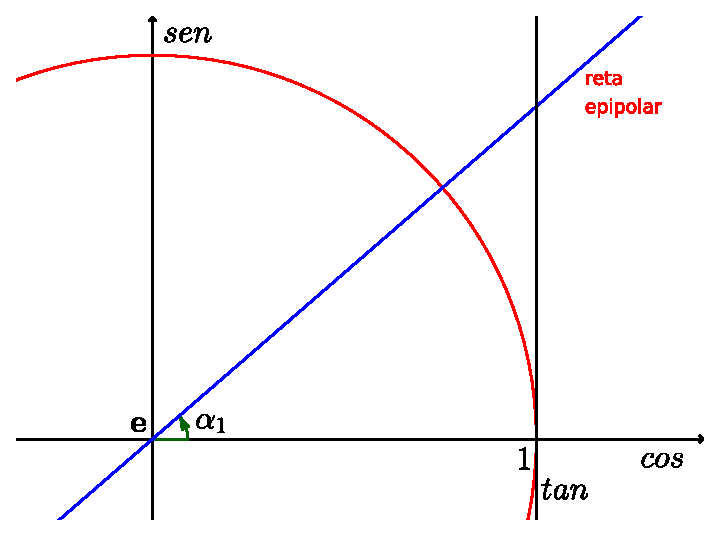
\includegraphics[scale=1]{reta-epipolar-alpha1}
\caption{\textit{Plano da imagem centrado em ${\bf e}$ com a reta epipolar parametrizada por $\alpha_1$.}}
\label{fig.reta-epipolar}
\end{figure}

Com essa conversão, deixamos de parametrizar as retas epipolares pelo eixo da tangente e passamos a parametrizar pelo círculo trigonométrico. Aqui temos um argumento para contagem dos graus de liberdade para fixarmos a relação entre retas epipolares, pois devemos determinar os dois epipolos (duas variáveis cada totalizando quatro graus de liberdade), e mais a matriz que representa a homografia (quatro variáveis mas apenas três graus de liberdade utilizando uma variável para fixar a escala). Portanto, precisamos de no mínimo sete restrições para determinarmos a relação entre duas imagens na geometria epipolar. 

Na nossa abordagem, consideramos o círculo trigonométrico com raio $1$ mas podemos estipular raios arbitrários $r_1$ e $r_2$ em cada uma das imagens que ajuda a garantir estabilidade numérica para a determinação dos coeficientes. Assim, obtemos a equação:

\begin{equation*}
a\,r_1\,sen\,\alpha_1\,r_2\,sen\,\alpha_2+b\,r_1\,sen\,\alpha_1\,r_2\,cos\,\alpha_2+c\,r_1\,cos\,\alpha_1\,r_2\,sen\,\alpha_2+d\,r_1\,cos\,\alpha_1\,r_2\,cos\,\alpha_2=0.
\end{equation*}

Em resumo, as vantagens dessa última representação é ser isotrópica e ter boa estabilidade numérica para escolhas convenientes de $r_1$ e $r_2$, e novamente  na representação matricial:

\begin{equation*}
(r_1\,cos\,\alpha_1\,,\,r_1\,sen\,\alpha_1)
\begin{bmatrix}
d&c\\
b&a
\end{bmatrix}
\begin{pmatrix}
r_2\,cos\,\alpha_2\\
r_2\,sen\,\alpha_2
\end{pmatrix}
=0
\end{equation*}

Uma outra forma de pensar sobre essa homografia, encontrada em \cite{Hartley2004}, é considerando que as retas epipolares estão perspectivamente relacionadas com centro em um ponto $Q$ na reta base, conforme a figura \ref{fig.retas-epi-hartley}.

\begin{figure}[!htb]
\centering
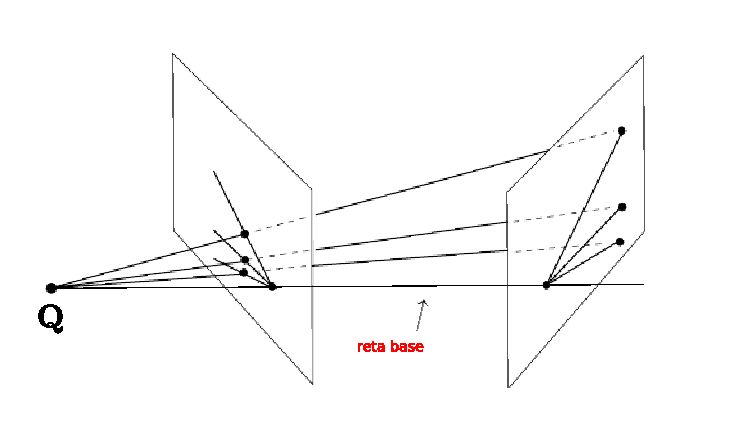
\includegraphics[scale=1]{retas-epipolares-hartley}
\caption{\textit{Retas epipolares com perspectiva centrada em $Q$ na reta base.}}
\label{fig.retas-epi-hartley}
\end{figure}


Suponha que $\lightrgb$ e $\lightrgb'$ sejam duas retas epipolares correspondentes, e ${\bf m}$ é uma reta qualquer que não passa pelo epipolo $\e$. O produto vetorial 

\begin{equation}
{\bf m}\times\lightrgb=\x\qquad\text{ou}\qquad\,[{\bf m}]_\times\,\lightrgb=\x,
\end{equation}
nos fornece o ponto $\x$ de interseção entre essas retas. Pela subseção \ref{sec.matriz-F} temos que

\begin{equation*}
\lightrgb'=F\,\x,
\end{equation*} 
assim, $\lightrgb$ é mapeada a $\lightrgb'$ através da relação 

\begin{equation*}
\lightrgb'=F\,[{\bf m}]_\times\,\lightrgb
\end{equation*}


Uma boa escolha para ${\bf m}$ é a reta $\e$, já que

\begin{equation*}
{\bf m}^\top\e=\e^\top\e\neq0,
\end{equation*}
então $\e$ é uma reta que não passa pelo epipolo $\e$ como desejado. Assim, a homografia da reta epipolar pode ser escrita como 

\begin{equation*}
\lightrgb'=F\,[\e]_\times\,\lightrgb.
\end{equation*}
O argumento é análogo para o mapeamento da segunda imagem para a primeira,

\begin{equation*}
\lightrgb=F^\top [\e']_\times\,\lightrgb'.
\end{equation*}\\

{\bf A matriz de calibração e a imagem da cônica absoluta.} Uma ferramenta algébrica bastante utilizada nessa abordagem de \citep{2503343} é a imagem da cônica absoluta (IAC em inglês) denotada por ${\bf \omega}$. Como a abordagem assume que as câmeras são calibradas, vamos mostrar que é possível obter a IAC em função da matriz de calibração da câmera $K$. Vamos determinar a homografia que faz o mapeamento do plano no infinito $\bpi_\infty$ para o plano da imagem na câmera. Se $\X_\infty\in\bpi_\infty$ então pode ser escrito na forma

\begin{equation*}
\X_\infty=({\bf d}^\top,0)^\top
\end{equation*} 
e é projetado por uma câmera geral $P=K\,[R|{\bf t}]$ como

\begin{equation*}
\begin{array}{rcl}
\x&=&P\,\X_\infty\\
&=&K\,[R|{\bf t}]\,({\bf d}^\top,0)^\top\\
&=&K\,R\,{\bf d}.
\end{array}
\end{equation*}
Portanto temos a relação

\begin{equation*}
\x=H\,{\bf d}
\end{equation*}
onde $H=K\,R$. Como a cônica absoluta $\Omega_\infty$ está contida no plano no infinito (contém pontos no infinito), ela pode ser projetada sob a homografia $H$ para computarmos sua imagem.
Sob uma homografia de ponto $\x\rightarrow H\,\x$, uma cônica se transforama de acordo com $C\rightarrow H^{-\top} C\,H^{-1}$, conforme a seção tal. De acordo com a seção tal $C=\Omega_\infty =I$, daí temos

\begin{equation*}
\begin{array}{rcl}
{\bf \omega}&=&H^{-\top}\Omega_\infty\,H^{-1}\\
&=&(K\,R)^{-\top}\,I\,(K\,R)^{-1}\\
&=&K^{-\top}R^{-\top}R^{-1}K^{-1}\\
&=&K^{-\top}K^{-1}
\end{array}
\end{equation*}
pois $R$ é uma matriz de rotação e portanto satisfaz $R^{-\top}R^{-1}=I$. Assim, de posse de uma câmera calibrada é simples obter a IAC.\\

{\bf As restrições Kruppa.} Para a correspondência entre duas cônicas ${\bf \omega}$ e ${\bf \omega'}$ podemos utilizar a restrição \textit{Kruppa}: as duas retas tangentes à ${\bf \omega}$ e passando por $\e$, estão relacionadas por uma homografia de reta epipolar às duas tangentes à ${\bf \omega'}$ passando por $\e'$. Na figura \ref{epipolar-kruppa} podemos observar as restrições epipolar e Kruppa simultaneamente.

\begin{figure}[!htb]
\centering
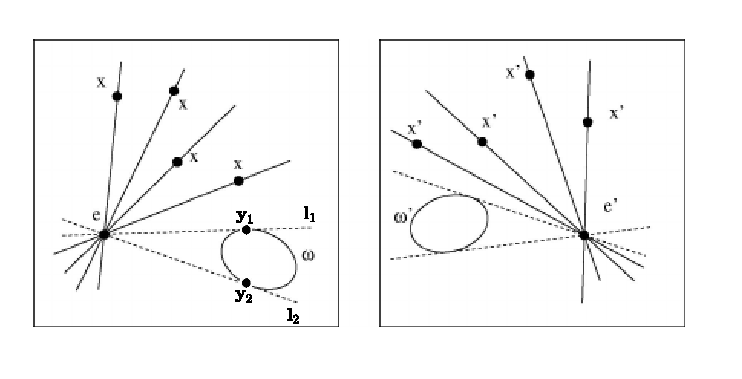
\includegraphics[scale=1.2]{restricao-epipolar-kruppa}
\caption{\textit{Retas epipolares tangentes às cônicas ${\bf \omega}$ e ${\bf \omega'}$.}}
\label{epipolar-kruppa}
\end{figure}

A restrição Kruppa foi originalmente introduzida por citar faugeras 92a (do hartley) e está relacionada com uma cônica contida num plano no espaco 3D e suas imagens nas câmeras $1$ e $2$, e é válida para cônicas gerais, mas aqui no nosso caso vamos tratar especificamente da cônica absoluta $\Omega_\infty$ contida no plano infinito $\bpi_\infty$ no espaco, e as imagens da cônica absoluta (IAC em inglês) ${\bf \omega}$ e ${\bf \omega'}$. Sendo ${\bf \omega}^*$ e ${{\bf \omega}^*}'$ as respectivas cônicas duais (definida por retas e com sigla DIAC em inglês), considere um plano passando pelo centro das duas câmeras e tangenciando essa cônica $\Omega_\infty$ no espaco. Por construção, esse plano vai projetar uma reta epipolar em cada imagem onde cada reta será tangente às imagens ${\bf \omega}$ e ${\bf \omega'}$ da cônica $\Omega_\infty$, observado na figura \ref{geometria-kruppa}. E suponha ainda que $\lightrgb_1$ e $\lightrgb_2$ sejam as retas tangentes à cônica ${\bf \omega}$ na primeira imagem conforme a figura \ref{epipolar-kruppa}. Com essas duas retas tangentes podemos construir uma cônica degenerada $D$ (posto $1$ ou $2$) da seguinte maneira:  

\begin{equation}\label{eq.def.con.deg}
D=[\e]_\times\,{\bf \omega}^*\,[\e]_\times \qquad \text{ou, como outra construção} \qquad D=\lightrgb_1\,\lightrgb_2^\top + \lightrgb_2\,\lightrgb_1^\top
\end{equation}

Para mostrar que $D$ é uma cônica (ponto) temos que verificar que é válida a relação $\y_1^\top D\,\y_1=0$, onde $\y_1\in\lightrgb_1$.

\begin{equation*}
\begin{array}{rcll}
\y_1^\top\,D\,\y_1&=&\y_1^\top [\e]_\times\,{\bf \omega}^*\,[\e]_\times\,\y_1&\\
&=&([\e]_\times\,\y_1)^\top {\bf \omega}^*\,[\e]_\times\,\y_1& \qquad [\e]_\times\,\text{é simétrica}\\
&=&\lightrgb_1^\top {\bf \omega}^*\,\lightrgb_1& \qquad\text{pois}\qquad\lightrgb_1=\e\times\y_1\\
&=&0&
\end{array}
\end{equation*}
onde a última passagem segue do fato de ${\bf \omega}^*$ ser dual. Analogamente, para a segunda definição de $D$:

\begin{figure}[!htb]
\centering
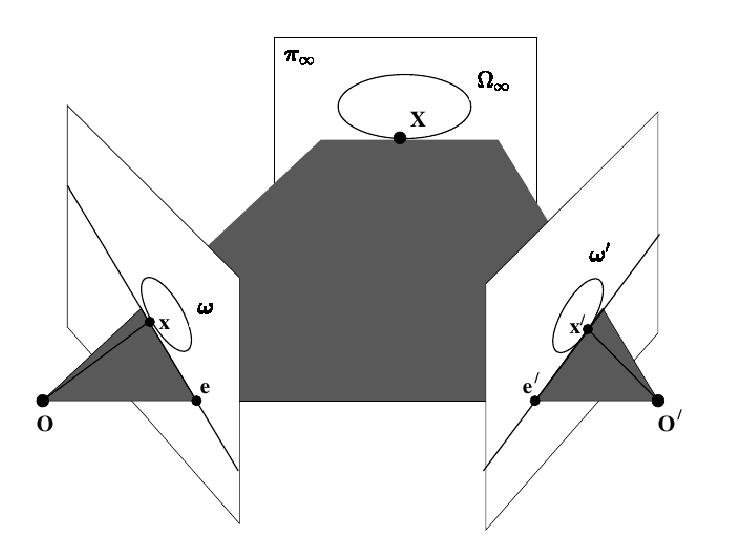
\includegraphics[scale=1.1]{geometria-kruppa}
\caption{\textit{Um plano epipolar tangenciando uma cônica no espaco 3D projeta retas epipolares que tangenciam as cônicas nos planos das imagens}.}
\label{geometria-kruppa}
\end{figure}

\begin{equation*}
\y_1^\top\,D\,\y_1=\y_1^\top \lightrgb_1\,\lightrgb_2^\top + \lightrgb_2\,\lightrgb_1^\top\y_1=0
\end{equation*}
pois como $\y_1\in\lightrgb_1$ então $\y_1^\top \lightrgb_1=\lightrgb_1^\top\y_1=0$. Observamos que o desenvolvimento anterior é análogo para $\lightrgb_2$.

Na segunda imagem, analogamente à primeira, $D'=[\e']_\times\,{{\bf \omega}^*}'\,[\e']_\times$ e se transforma de acordo com $D'=H_\infty^{-\top}D\,H_\infty^{-1}$ na seção tal. O símbolo $\infty$ se deve ao fato de que a homografia foi deduzida de maneria similar àquela da seção  \ref{sec.homografia}, apenas com a diferença de ter sido com base no plano no infinito. Assim:

\begin{equation}
\begin{array}{rcll}
[\e']_\times\,{{\bf \omega}^*}'\,[\e']_\times&=&D'&\\
&=&H_\infty^{-\top}D\,H_\infty^{-1}&\\
&=&H_\infty^{-\top}[\e]_\times\,{\bf \omega}^*\,[\e]_\times\,H_\infty^{-1}&\qquad\text{pois}\qquad D=[\e]_\times\,{\bf \omega}^*\,[\e]_\times\\
&=&F\,\omega^* F^\top,&
\end{array}
\end{equation}
onde $F=H_\infty^{-\top}\,[\e]_\times$ conforme a subseção \ref{sec.matriz-F}. 


Como \cite{2503343} aplica uma transformação no plano da imagem para que os objetos geométricos tenham as mesmas coordenadas nos dois planos, temos que $\omega^*$ e ${\omega^*}'$ têm as mesmas coordenadas, assim a relação

\begin{equation*}
[\e']_\times\,{{\bf \omega}^*}'\,[\e']_\times=F\,\omega^* F^\top
\end{equation*}
se transforma em 

\begin{equation}\label{eq.kruppa}
[\e']_\times\,{\bf \omega}^*\,[\e']_\times=F\,\omega^* F^\top.
\end{equation}



Da relação \ref{eq.kruppa} são extraídas as duas equações quadráticas independentes eliminando-se o fator de escala, onde tais equações são conhecidas como as restrições de Kruppa. 




De acordo com \cite{kneebone}, podemos escolher as coordenadas projetivas de forma que os quatro pontos também tenham as mesmas coordenadas em cada imagem. Ou seja, podemos assumir que ${\bf x}_i = {\bf x'}_i$ pensando nos dois planos de imagem como registrados no mesmo sistema de coordenadas. Desta forma, a restrição epipolar pode ser convertida em: os epipolos ${\bf e}$ e ${\bf e'}$, que obedecem a restrição epipolar, devem estar alojados numa cônica $B$ e, reciprocamente, dois epipolos ${\bf e}$ e ${\bf e'}$ que são concônicos com quatro pontos na imagem satisfazem a restrição epipolar. Esta cônica $B$ será bastante importante durante a abordagem pois, se os dois epipolos são concônicos com os quatro pontos na imagem, figura \ref{pontos-conconicos}, existe uma \textit{única} homografia de reta epipolar que faz a relação das quatro retas através ${\bf e}$ com as quatro retas através ${\bf e'}$. 

\begin{figure}[!htb]
\centering
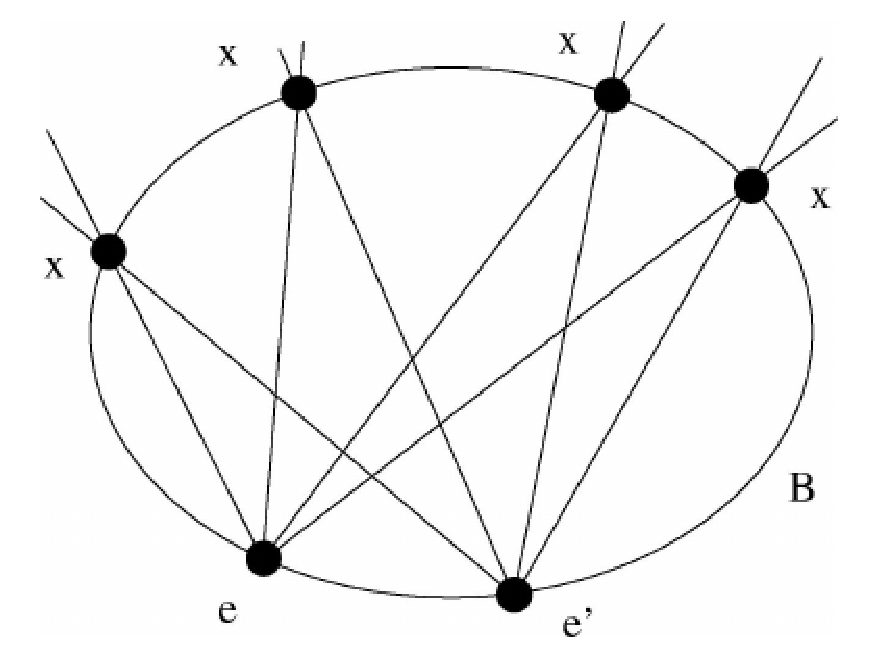
\includegraphics[scale=.85]{pontos-conconicos}
\caption{\textit{Epipolos concônicos com os quatro pontos na imagem produzem homografia única.}}
\label{pontos-conconicos}
\end{figure}

Note que podemos parametrizar o feixe de retas passando por ${\bf e'}$ (ou ${\bf e}$) por pontos pertencentes à cônica $B$, pois retas correspondentes nos dois feixes intersectam $B$ no mesmo ponto. Desta forma, a restrição Kruppa pode ser traduzida como: as restrições de calibração são equivalentes à condição de que as duas retas tangentes à cônica ${\bf \omega}$ e passando por ${\bf e}$, intersectam a cônica $B$ nos mesmos dois pontos adicionais que as retas tangentes à ${\bf \omega'}$ e passando por ${\bf e'}$. Isto é, as projeções de ${\bf \omega}$ e ${\bf \omega'}$ em $B$, através dos respectivos epipolos, devem coincidir. Essa construção geométrica pode ser visualizada na figura \ref{omega-B} e será a fundação para o resto da abordagem. 

\begin{figure}[!htb]
\centering
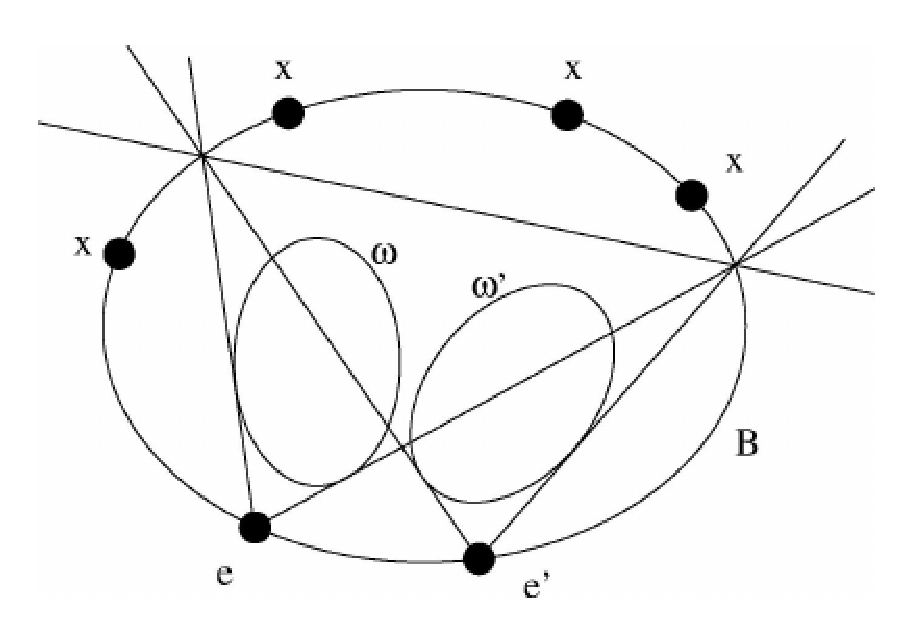
\includegraphics[scale=.85]{projecao-omega-B}
\caption{\textit{Os pontos de interseção das tangentes com a cônica $B$ coincidem, ocasionando a coincidência das projeções das cônicas ${\bf \omega}$ e ${\bf \omega'}$ na cônica $B$.}}
\label{omega-B}
\end{figure}

Podemos pensar na representação da projeção de  ${\bf \omega}$ e ${\bf \omega'}$ em $B$ como a reta que liga os dois pontos de interseção das tangentes com $B$. Essa reta que liga os dois pontos de interseção, de acordo com a projeção de ${\bf \omega}$ através do epipolo ${\bf e}$ é representada por $({\bf \omega}\diamond B)\,{\bf e}$, e a cônica $({\bf \omega}\diamond B)$ é definida como:

\begin{equation}
(\omega \diamond B)\equiv 2\,B\,\omega^*B - tr(\omega^*\,B)\,B,
\end{equation}
onde $\omega^*$ é a matriz adjunta de $\omega$.

Note que a reta $(\omega \diamond B)\,{\bf e}$ é a reta polar de ${\bf e}$ com relação à cônica $(\omega \diamond B)$. Está sendo usada a relação polo-polar definida pelo locus da cônica $(\omega \diamond B)$ para executar a projeção. Já que os pontos de interseção das tangentes com $B$ são os mesmos para as duas cônicas $\omega$ e $\omega'$, pode ser verificado que, dado que ${\bf e}$ e ${\bf e'}$ são concônicos com quatro pontos na imagem, a restrição Kruppa é equivalente à restrição de que as retas polares $(\omega \diamond B)\,{\bf e}$ e $(\omega' \diamond B)\,{\bf e'}$ coincidem.


Note que $(\omega \diamond B) = B\,(\omega \cdot B)$ se definirmos a homografia

\begin{equation}
(\omega \cdot B) \equiv 2\,\omega^*\,B - tr(\omega^*\,B)\,I,
\end{equation}
onde está sendo ``cancelado" $B$ na definição de $(\omega \diamond B)$. 


Como $(\omega' \diamond B)\,{\bf e}$ e $(\omega' \diamond B)\,{\bf e'}$ coincidem e usando a equivalência anterior, podemos demonstrar que 

\begin{equation}
(\omega' \cdot B)\,{\bf e'} \sim (\omega \cdot B)\,{\bf e}
\end{equation} 
(onde $\sim$ significa igualdade a menos da escala) o que implica num mapeamento de sétimo grau 

\begin{equation}
{\bf e} \rightarrow {\bf e'} \sim (\omega' \cdot B)^*\,(\omega \cdot B)\,{\bf e}.
\label{funcao-de-e}
\end{equation}

No artigo também é domonstrado que a restrição Kruppa disponibiliza quatro soluções (dois pares de soluções coincidentes) para cada ${\bf e}$, e as soluções são as interseções (figura \ref{inter-B-C}) de $B$ com a cônica 

\begin{equation}
C \equiv (\omega \cdot B)^\top\,(\omega' \cdot B)^{*\,\top}\,B\,(\omega' \cdot B)^*(\omega \cdot B).
\end{equation}

\begin{figure}[!htb]
\centering
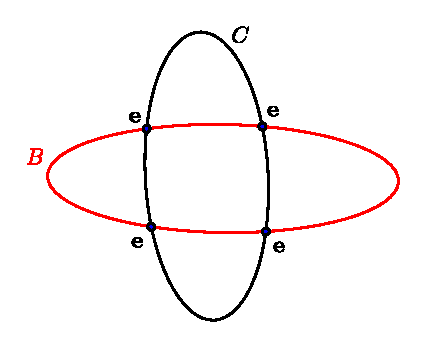
\includegraphics[scale=.6]{intersecao-C-B}
\caption{\textit{Epipolos que satisfazem as restrições de projeção e de calibração podem ser encontrados como as interseções das cônicas B e C.}}
\label{inter-B-C}
\end{figure}

Um epipolo ${\bf e}$ que gera uma cônica $B$ satisfaz à equação de décimo-sexto grau

\begin{equation}
{\bf e}^\top\,C\,{\bf e} = 0
\label{dezesseis}
\end{equation}
se, somente se, ele satisfaz às restrições de projetividade e de calibração. No caso em que a cônica $B$ pode se degenerar em um par de retas, a homografia $(\omega \cdot B)$ permuta as retas do par e assim, a equação \ref{dezesseis} descreve também seis retas passando por cada par dos quatro possíveis epipolos na imagem. Algebricamente, isso significa que a equação \ref{dezesseis} tem $|B|$ como um fator. Na figura \ref{plot-C} podemos observar duas plotagens da curva de dezesseis graus, uma com e outra sem a visualização dessas seis retas.

\begin{figure}[!htb]
\centering
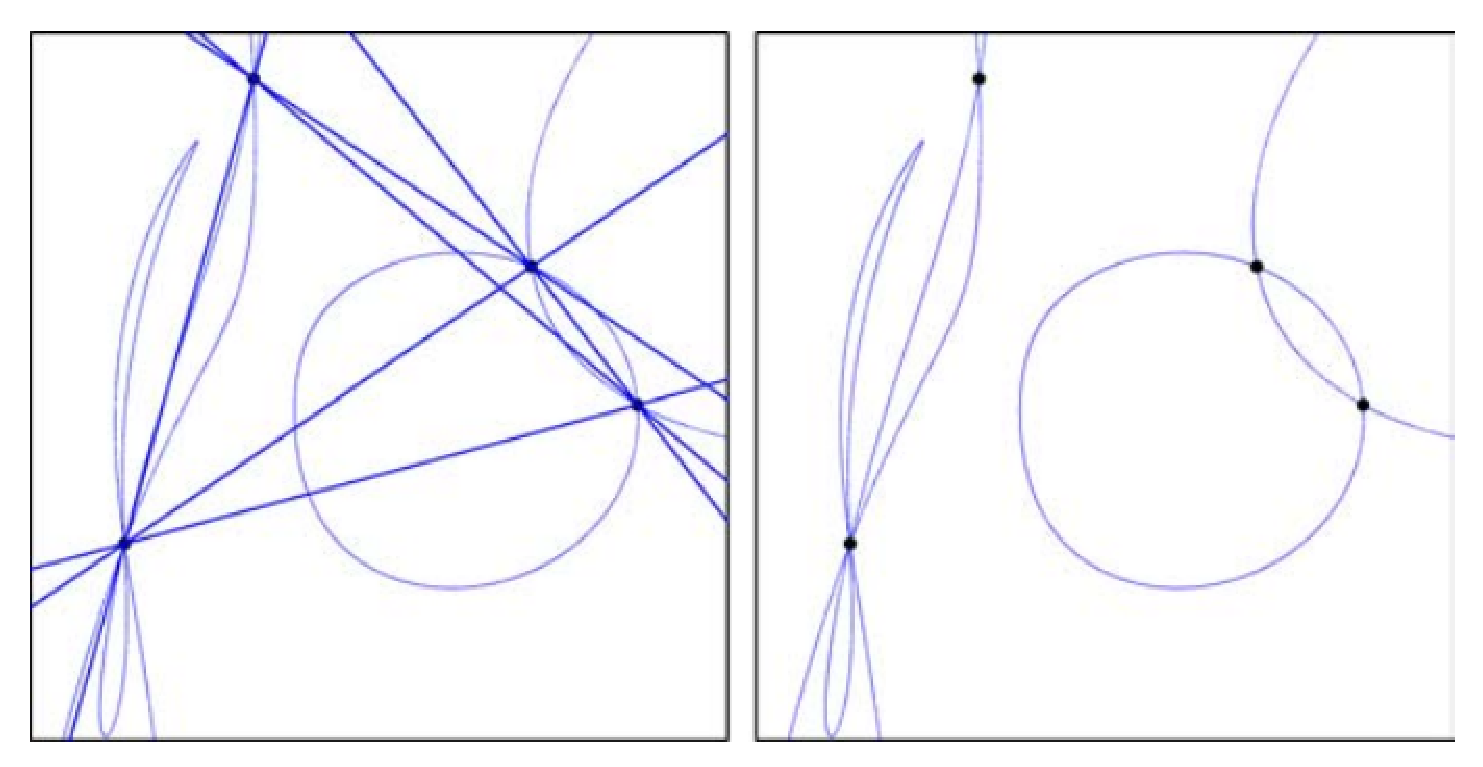
\includegraphics[scale=.6]{plotagem-C}
\caption{\textit{Podemos observar o lugar geométrico dos possíveis epipolos definido pela equação de décimo-sexto grau, a qual define (alem das curvas) as possíveis seis retas. A direita, a mesma imagem sem as retas.}}
\label{plot-C}
\end{figure}

Qualquer epipolo ${\bf e}$ para o qual $|B|\ne0$ satisfaz as restrições de projetividade e calibração se, e somente se, ${\bf e}$ satisfaz a equação de décimo grau remanescente de $e^\top\,C\,e=0$, ou seja, a equação restante após a eliminação do $|B|\ne0$. Geometricamente, temos que os pontos não podem se alojar em quaisquer das seis retas por conta da restrição de calibração. É possível remover $|B|\ne0$ da equação \ref{dezesseis} para se chegar à equação de décimo grau e o trabalho é algebricamente pesado mas também pode ser inteiramente encontrado em \cite{kneebone}. A curva de décimo grau é descrita pela equação

\begin{equation}
e^\top\,G\,e=0,
\label{dez}
\end{equation}
onde 
\begin{equation}
G=4\,U^\top\,D'^*\,B^*\,D'^*\,U-4\,t'^2\,B\,D\,D'^*\,(D\,B-t\,I)+s\,D^*-t^2\,t'^2\,D'^*
\label{conica-G}
\end{equation}
com as definições:

\begin{equation}
\begin{array}{rcl}
D&\equiv&\omega^*,\\
t&\equiv&tr(D\,B),\\
U&\equiv&(\omega \cdot B)\,\,\, \text{e}\\
s&=&(16\,|B|\,|D'|\,t'+t'4-4\,t'2\,tr(B*\,D'*)).
\end{array}
\end{equation}

A partir das consideraçoes feitas até aqui, podemos expor o principal resultado de \cite{kneebone}, o qual afirma que um ponto é um candidato a epipolo de acordo com as restrições de projetividade e calibração se, e somente se, satisfaz a equação de décimo grau definida em \ref{dez}. O que é equivalente ao fato de que ${\bf e}$ deve se alojar na cônica $G$ definida em \ref{camera-G}. Para um epipolo ${\bf e}$ qualquer na curva de décimo grau, o outro epipolo ${\bf e'}$ é calculado pela função de sétimo grau ${\bf e'} \sim U'*\,U\,{\bf e}$, dada em \ref{funcao-de-e}. Na figura \ref{curva-10} observamos alguns exemplos de curvas de décimo grau com seus possíveis epipolos. 

\begin{figure}[!htb]
\centering
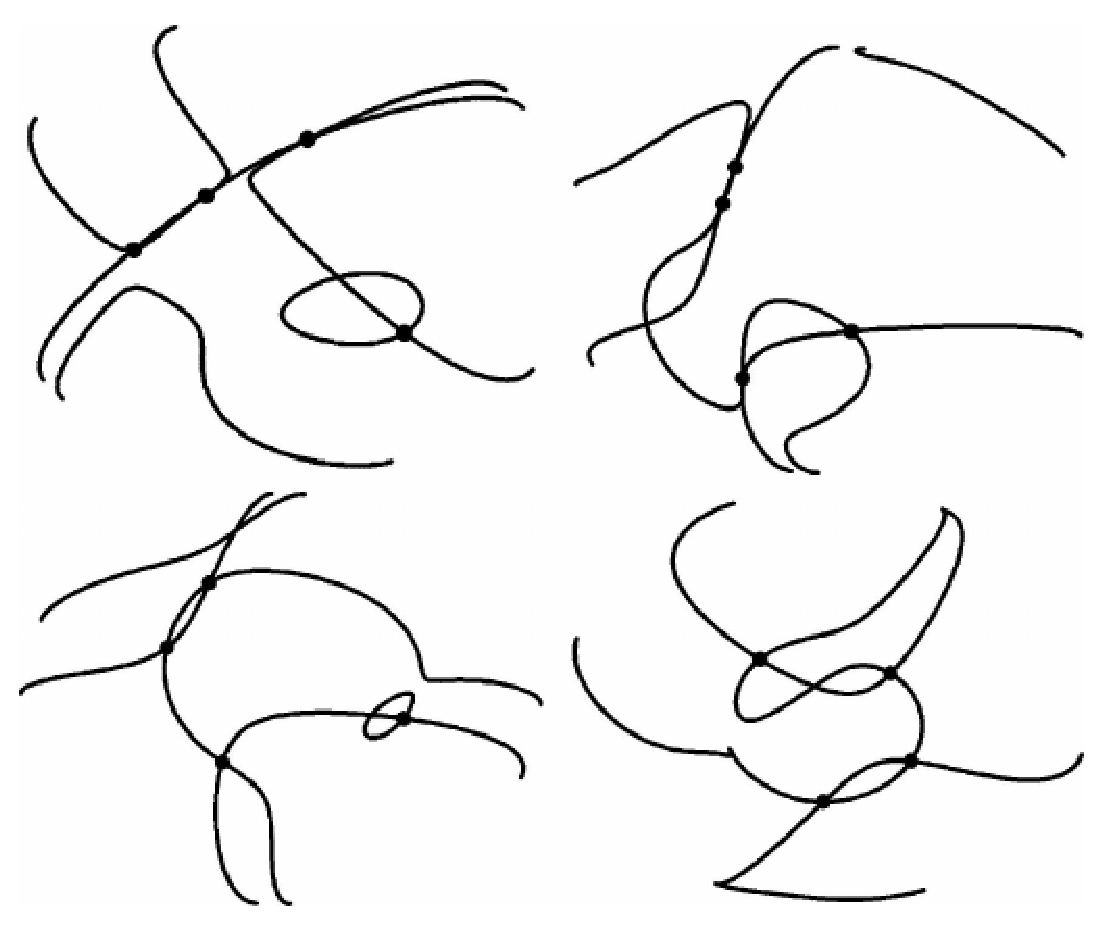
\includegraphics[scale=.85]{ex-curva-10}
\caption{\textit{Quatro exemplos de curvas de decimo grau definidas pela equaçao \ref{dez}, juntamente com seus respectivos epipolos.}}
\label{curva-10}
\end{figure}

Dado um ponto na curva de décimo grau, é importante verificar se o mesmo satisfaz a restrição de orientação, que é o fato de o correspondente ponto 3D no espaço situar-se em frente ao plano das duas imagens, conforme retratado na figura \ref{retr-orien}. Ou seja, o ponto no espaço 3D deve situar-se na metade da frente dos raios emanados de seus respectivos pontos nas duas imagens. Dado um epipolo ${\bf e}$ numa imagem, ${\bf e'}$ fica unicamente determinado pela equação \ref{funcao-de-e} na outra imagem. Após determinado o par de epipolos, a homografia da linha epipolar é unicamente definida pela correspondência desses pontos e assim determinamos a matriz essencial. Se ignorarmos uma diferença de escala considerando que a linha base que liga as duas câmeras tem comprimento unitário, temos que existem quatro configurações para a posição das duas imagens num sistema 3D. A restrição projetiva é satisfeita em quisquer dessas quatro configurações, pois os dois raios emanados do par de pontos correspondentes nas duas imagens continuam coplanares e devem se interseptar num ponto comum. A restrição de orientação é satisfeita exatamente quando os quatro pares de pontos correspondentes indicam a mesma configuração. Podemos dividir a restrição de orientação em duas partes: primeiro quando a homografia de reta epipolar é orientada, ou seja, quando os dois raios passando pelo par de pontos correspondentes nas imagens, estão no mesmo semiplano definido pela reta base onde se encontram as imagens (será chamada restrição de orientação epipolar); e segundo, a condição de que as duas metades dos raios que se projetam para a parte da frente devem convergir para um ponto comum (será chamada restrição de convergência).  

\begin{figure}[!htb]
\centering
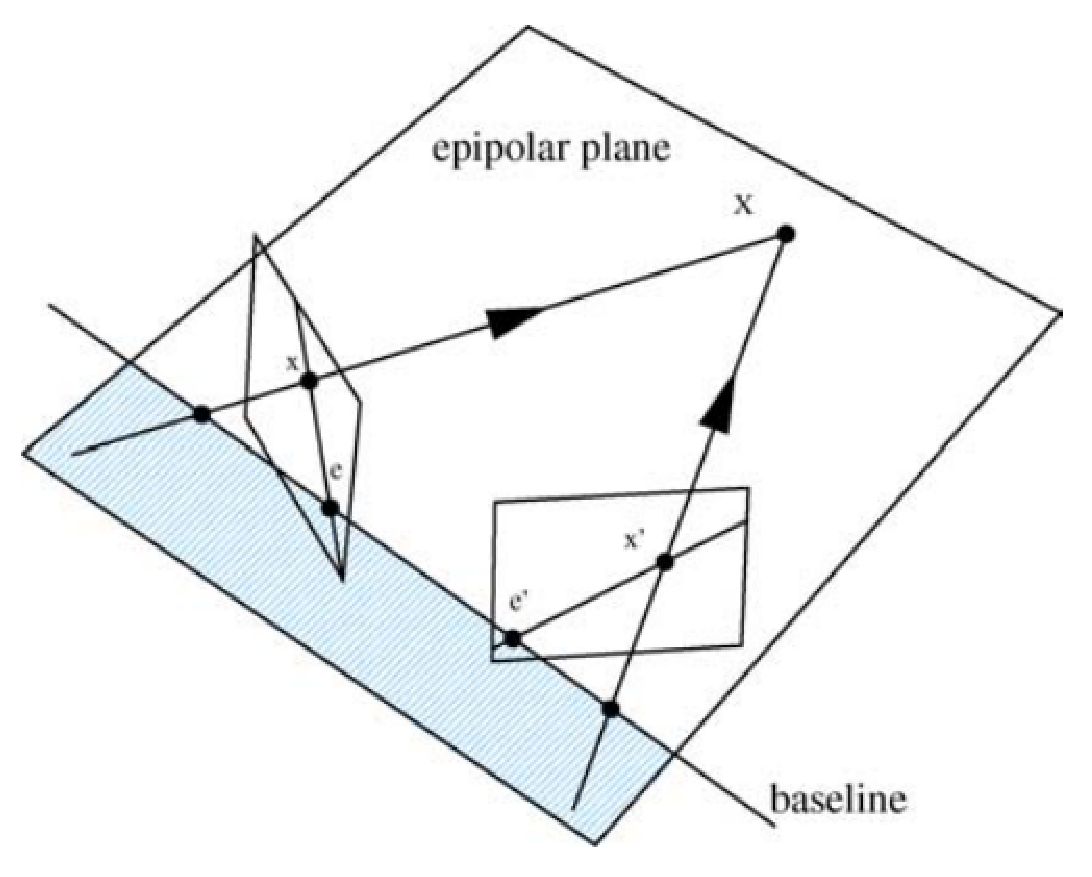
\includegraphics[scale=.85]{restricao-orientacao}
\caption{\textit{A restrição de orientação é simplesmente o fato de que o ponto no espaço 3D deve estar na parte da frente dos respectivos raios emanados de cada imagem.}}
\label{retr-orien}
\end{figure}

A restrição de convergência deve garantir que raios retroprojetados de cada imagem devem convergir. Isso não acontece somente se os raios forem paralelos e, uma forma de parametrizar, é através do ângulo formado entre o ponto na primeira imagem ${\bf x}$ e ${\bf e}$, e o ângulo entre o ponto na segunda imagem ${\bf x'}$ e ${\bf e'}$. Como a reta base passa por ${\bf e}$ e ${\bf e'}$, se os ângulos com os respectivos pontos forem iguais, os dois raios serão paralelos e não ocorrerá a convergência.


{\bf Aplicação da teoria no caso trifocal, com quatro pontos e três imagens.} As novidades do artigo se encontram, basicamente, no tipo de reconstrução 3D para duas imagens. A aplicação a seguir segue o padrão, até então convencional, de projetar as reconstruções na terceira imagem e minimizar o erro em relação aos dados já disponíveis. Assim, dados quatro pontos numa imagem e suas respectivas correspondências em outras duas imagens (todas com as câmeras calibradas), podemos escolher duas dessas imagens para traçarmos a curva de décimo grau de acordo com a esolha de um parâmetro $\theta$ que irá definir a cônica $B$, do feixe de cônicas, a ser utilizada.  Dada $B$ podemos calcular a cônica $G$ a partir da equação \ref{conica-G} como uma função de $B$, e as interseções de $B$ e $G$ podem ser determinadas como a solução de uma equação de quarto grau confrome descrito no apêndice do artigo. Assim, temos quatro soluções para   ${\bf e}$ e cada solução pode ser usada para calcular ${\bf e'}$ na segunda imagem de acordo com a equação \ref{funcao-de-e}. Note que para cada parâmetro $\theta$ teremos, a partir daqui, dezesseis caminhos a seguir. Com os epipolos encontramos a homografia da reta epipolar  e daí, a matriz essencial das duas imagens para cada uma das soluções. Existem vários métodos para reconstrução à partir da triangulação usando duas imagens, como por exemplo, \cite{nister5p2v} e \cite{Fabbri:Kimia:IJCV2015}. Conseguidas as reconstruções dos pontos 3D, existem também vários outros métodos de obtenção da câmera ralativa à terceira imagem, como por exemplo \cite{haralick} e \cite{bib:kuang}. Usados três pontos 3D para determinar a câmera da terceira imagem, podemos usar o quarto ponto para ser projetado na terceira imagem e comparar o resultado com o dado já obtido. Ou seja, para cada escolha do parâmetro $\theta$ (ou da cônica $B$), o procedimento consiste em minimizar um erro na imagem. Como o problema é supra restringido por um grau de liberdade, com os ruídos das correspondências, o valores encontrados para a reprojeção do quarto ponto não coincidirá com o dado observado mesmo que usada a correta solução. Como para cada $\theta$ escolhido teremos dezesseis configurações de câmera da terceria imagem e dezesseis reporjeções, todas essas reprojeções definem uma complexidade enorme de curvas na terceira imagem. Na figura \ref{curvas-f(theta)} é dada uma ideia da dificuldade extrema do problema envolvendo três imagens e quatro pontos. 

\begin{figure}[!htb]
\centering
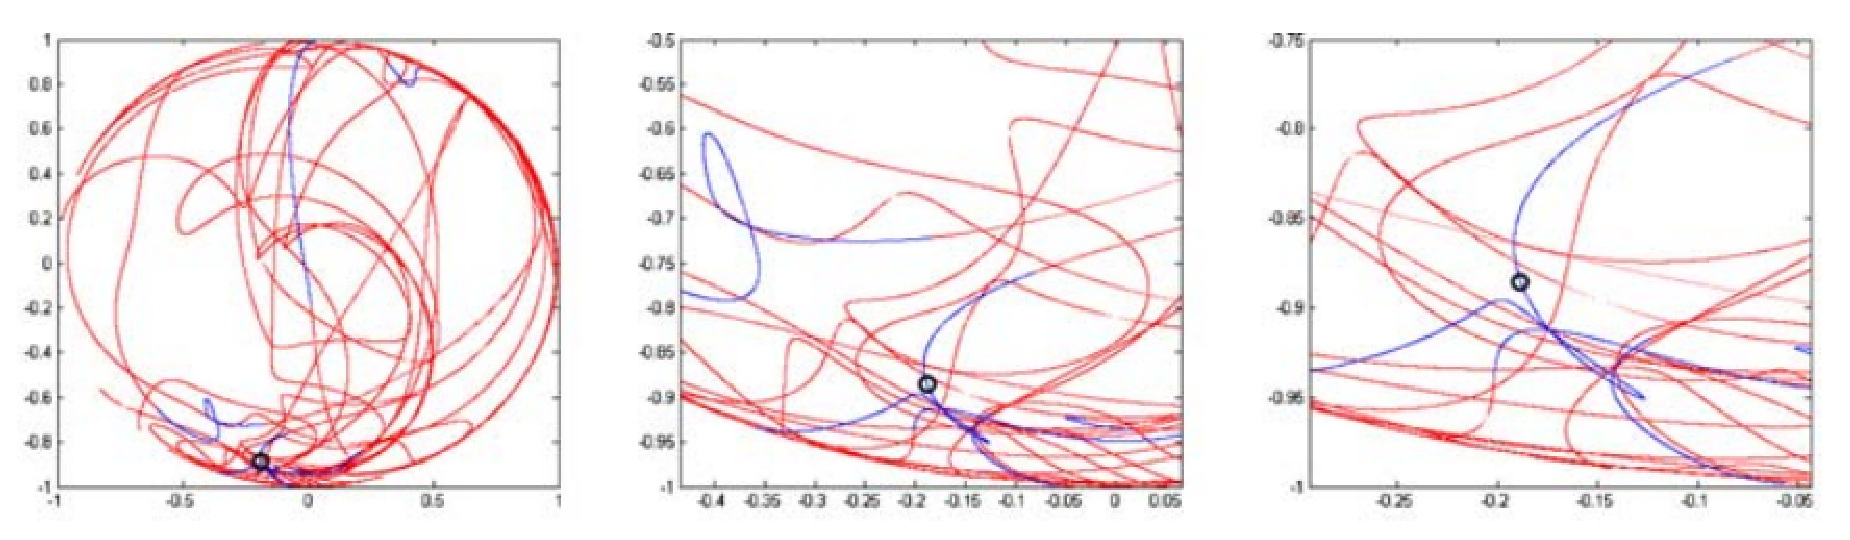
\includegraphics[scale=.52]{varias-curvas-f-theta}
\caption{\textit{A reprojeçao do feixe de conicas na terceira imagem e do quarto ponto reconstruido nos da uma ideia da dificuldade do problema de 3 imagens com quatro pontos.}}
\label{curvas-f(theta)}
\end{figure}

Para um grupo aleatório de quatro pontos, em geral a projeção da curva de décimo grau não passará pelos pontos. Antes de iniciar os cálculos, os pontos são co-registrados por uma homografia que será usada para transformar o DIAC  da segunda imagem no sistema de coordenadas da primeira. Existem várias maneiras de parametrizar o feixe de cônicas e uma delas é escolher duas cônicas dentre as degeneradas como base para o feixe.





\subsubsection{Abordagem de Schimd e Zisserman}

Este artigo lida com o problema de encontrar correpondências entre seguimentos de curvas quando temos diponíveis duas ou três imagens de câmeras deconhecidas. A matriz fundamental e o tensor trifocal são facilmente computados através de pontos de interesse mais o uso do RANSAC, mas os parâmetros intrínsecos não precisam necessariamente ser conhecidos. A abordagem clássica é descartar esses pontos de interesse e usar a geometria da câmera em estágios subsequentes de associação estéreo, para eliminar a ambiguidade entre pontos correspondentes ao longo da linha epipolar. Com duas imagens, o método padrão é usar a restrição epipolar para computar pontos correspondentes, o qual limita os canditados a estarem numa região estreita, e o uso de correleção cruzada normalizada, obtida a partir de fotometria, para restringir mais ainda nossas escolhas dos pontos. 

No artigo são analisados dois casos, binocular e trinocular, para responder a uma questão principal: existe alguma restrição adicional quando não utilizamos pontos mais sim pontos-tangentes ou geometria de curvas em geral disponíveis?\\

\noindent {\bf O Caso Binocular}

A busca por correspondências usando correlação fotométrica pode ser significantemente reduzida usando geometria de curvas (sem a utilização de contornos oclusos) numa pequena vizinhança. Considere uma aproximação de primeira ordem (planar) para a superfície de um objeto no qual aloja-se uma curva 3D. A correspondência entre as projeções desse plano em duas imagens são descritas por uma homografia de 8 parâmetros livres. É sabido que a matriz fundamental, que contém informações da geometria epipolar, fornece 5 restrições, o que reduz para 3 os graus de liberdade da homografia. Assim, o fato de que um ponto está associado a um outro ponto na reta epipolar já está sendo considerado nos cálculos. Dados alguns pontos correspondentes num fragmento de curva ao longo da linha epipolar, cada par de correspondência fornece duas restrições nas variáveis desconhecidas: como as curvas devem ser mapeadas umas nas outras, (i) a posição ao longo da linha epipolar define uma variável, já que o plano 3D é forçado a passar pelo ponto 3D reconstruído a partir dessa informação (a menos de uma homografia 3D). Assim, resta uma família de um parâmetro que pode ser otimizado usando o grau da correlação fotométrica. Dentre a família de um parâmetro de solução restante, os autores propuseram que, no lugar de otimizar através de correlação fotométrica, podemos apenas escolher o plano que coincide com o plano osculante da curva, o qual pode ser determinado usando a curvatura dos pontos correspondentes. Isto é apenas uma heurística, um método construtivo, onde não há garantia de que se trata da tangente à superfície, mesmo se a curva é plana. Contudo, empiricamente os autores expuseram que essa solução é boa o suficiente para criar uma fila ordenada das associações mesmo considerando os casos acima.

A questão de como conseguir um plano osculante (e a homografia associada a ele) foi a motivação para chegar a um resultado de interesse geral. Sabemos, através da posição e curvatura das extremidades correspondentes em duas imagens, que é possível estimar, unicamente, o plano osculante a uma curva se a calibração da imagem é completamente conhecida. Se apenas a matriz fundamental é conhecida, o plano osculante pode ser encontrado a menos da ambiguidade projetiva somente, mas a homografia associada a ele pode ser completamente determinada, o que é estudado nesse artigo.

\noindent {\bf O Caso Trinocular}

Os autores também propuseram um método para transferir a curvatura de duas imagens para uma terceira, dado um tensor trifocal (a calibração completa não é necessária). A interpretação da fórmula dada é usar o plano reconstruído a partir de duas imagens (conhecido a menos de uma ambiguidade projetiva 3D), e usá-lo para conseguir uma homografia relacionando as duas primeiras imagens com a terceira (sendo esta homografia independente dos parâmetros intrínsecos). Esta homografia define, então, a correspondência de pontos de quaisquer das duas primeiras imagens para a terceira. Faugeras e Robert foram os primeiros a proporem a transferência de curvatura a partir de duas imagens não calibradas para uma terceira, mas eles usaram par de matrizes fundamentais. O enriquecimento adicionado ao método de Faugeras proposto por Chimd e Zisserman é numericamente estável e imune a erros na interseção de linhas epipolares, que podem ser colineares ou aproximadamente colineares. O tensor trifocal manipula esses casos sem qualquer imprecisão.\\

\noindent {\bf Passo para um Sistema Prático} 

\begin{itemize}
\item Começar com a detecção de extremidades relacionadas em duas ou três imagens, e tentar associar fragmentos de curvas por inteiros.
\item Num primeiro estágio, considere apenas curvas alojadas no raio das linhas epipolares de cada uma das outras curvas, e têm tangências epipolares consistentes.
\item Num segundo estágio, tente encontrar fragmentos correspondentes de supostas curvas correspondentes através da integração do custo de extremidade-a-extremidade com possibilidade de associar fragmentos.
\item Usando apenas a geometria diferencial de curvas ganha-se restrições através de supostas extremidades associadas na terceira imagem. Isto funciona mesmo quando os parâmetros intrínsecos são desconhecidos, mas a ambiguidade permanece.
\item Restrições adicionais podem ser encontradas usando as aparências.
\item Para cada suposta associação, encontre um grupo de correlações no espaço gerado por um parâmetro se as curvaturas das associações são poucas (somente tangentes são utilizadas), ou não use buscas (planos osculantes) se as curvaturas acima são limites.
\item Um esquema das melhores escolhas dentre todas direciona para as associações finais.
\end{itemize}
